\documentclass[]{mediator_sp_hc}
\pdfoutput=1
%% -----------------------------------------------------------------
%% tento subor ma kodovanie ISO 8859-2 (latin2)
%%
%% na kompilaciu pouzivajte format pdfcslatex 
%%
%% vytvorene distribuciou texlive 2009-7
%% -----------------------------------------------------------------
\usepackage{lmodern,textcase}
\usepackage{slovak}\renewcommand{\figurename}{Obr�zok}
\def\refname{Zoznam pou�itej literat�ry}
\usepackage{latexsym}
\usepackage{dcolumn} % zarovnanie cisiel v tabulke podla des. ciarky
\usepackage{hhline}
\usepackage{amsmath}
\usepackage{nicefrac} % pekne zlomky
\usepackage{upgreek} % napr. $\upmu\mathrm{m}$ pre mikrometer ...
\usepackage[final]{showkeys}%color%notref%notcite%final
\usepackage[slovak,noprefix]{nomencl}
\makeglossary % prikaz na vytvorenie suboru .glo
\usepackage{parskip}% 'zhusti' polozky obsahu
\usepackage{comment}
\usepackage{listings}
\lstset{language=Java}

\usepackage{multirow}
\usepackage{booktabs}
%\usepackage{mathptmx} % pismo 'times' aj v matematike
\usepackage{amsmath}
%\usepackage{textcomp}

\usepackage{sverb}
\usepackage{alltt}
\usepackage{verbatim}
%nastavi male pismo pre vsetky verbatimy
\makeatletter 
\g@addto@macro\@verbatim\scriptsize
\makeatother 

\usepackage{amsmath,amssymb,amsfonts,textcomp}
\usepackage{color}
\usepackage{array}
\usepackage{supertabular}
\usepackage{hhline}
\usepackage{rotating}
\usepackage{textcomp}
%%
%\usepackage[dvips]{graphicx}
%\DeclareGraphicsExtensions{.eps}
%\usepackage[pdftex]{graphicx}
\DeclareGraphicsExtensions{.pdf,.png,.jpg,.mps}
\graphicspath{{figures/}} % priecinok na obrazky
%%
%% Cislovane citovanie
\usepackage[numbers]{natbib}
%%
%% Citovanie pod�a mena autora a roku
%\usepackage{natbib} \citestyle{chicago}
% -----------------------------------------------------------------
%% tla� !!!
\usepackage[pdftex,unicode=true,bookmarksnumbered=true,
bookmarksopen=true,pdfmenubar=true,pdfview=Fit,linktocpage=true,
pageanchor=true,bookmarkstype=toc,pdfpagemode=UseOutlines,
pdfstartpage=1]{hyperref}
\hypersetup{%
baseurl={http://www.tuke.sk/sevcovic},
pdfcreator={pdfcsLaTeX},
pdfkeywords={Sprostredkovanie, Medi\'ator, IPFIX, SLAMeter, BasicMeter},
pdftitle={Syst\'emov\'a pr\'iru\v{c}ka Mediator v1.0},
pdfauthor={Bc. Rastislav Kudla},
pdfsubject={Diplomov\'a pr\'aca}
} 

%\setlength{\parindent}{10mm}
%% nehodiace zakomentujte !
\dippraca{Diplomov� pr�ca}
%\bakpraca{Bakal�rska pr�ca}
%%
\nazov{Aplika�n� r�mec pre sprostredkovanie IPFIX spr�v v n�stroji SLAmeter}
%% ked praca nema 'podnazov' zakomentujte nasledujuci riadok
%% alebo polozku nechajte prazdnu
\podnazov{}
\klucoveslova{IPFIX, Sprostredkovanie, Medi�tor, Kolektor, Export�r, SLAmeter, BasicMeter, MONICA}
\jazyk{slovensk�}
\titul{In�inier}
\univerzita{Technick� univerzita v~Ko�iciach}
\university{Technical University of Ko�ice}
\fakulta{Fakulta elektrotechniky a informatiky}
\skratkafakulty{FEI}
\faculty{Faculty of Electrical Engineering and Informatics}
\katedra{Katedra po��ta�ov a informatiky}
\skratkakatedry{KPI}
\department{Department of Computers and Informatics}
\odbor{Informatika}
\specializacia{Informatika}


%priloha
%\kategoria{Pr�loha B}
%nazov prilohy
%\dekan{SYST�MOV� PR�RU�KA JXColl v3.5}
%rok prilohy
%\osnova{ 2010}

\autor{Bc.~Rastislav~Kudla}

\veducikatedry{doc.~Ing.~Jaroslav~Porub�n, PhD.}
\veduciprace{Ing.~Peter~Feci�ak,~PhD.}
\konzultanta{Ing.~Adri�n~Pek�r}
\konzultantb{}
\osnova{}
\zoznamodplit{}
\rozsahprace{}
\title{IPFIX Mediation Framework of the SLAmeter Tool}
\subtitle{}
\keywords{IPFIX, Mediation, Mediator, Collector, Exporter, SLAmeter, BasicMeter, MONICA}
\datumzadania{20. 1. 2012}
\datumodovzdania{29. 4. 2013}
\datumobhajoby{22. 5. 2013}
\mesto{Ko�ice}
\cpriloha{Pr�loha A}
\tpriloha{SYST�MOV� PR�RU�KA Mediator v1.0}

\pocetstran{\pageref{page:posledna}}


\begin{document}
\renewcommand\theHfigure{\theHsection.\arabic{figure}}
\renewcommand\theHtable{\theHsection.\arabic{table}}
\bibliographystyle{dcu}

\titulnastrana

\thispagestyle{empty}
\bigskip
\begin{quote}
    Copyright \copyright{}  2013  Rastislav Kudla.
    Permission is granted to copy, distribute and/or modify this document
    under the terms of the GNU Free Documentation License, Version~1.3
    or any later version published by the Free Software Foundation;
    with no Invariant Sections, no Front-Cover Texts, and no Back-Cover Text.
    A~copy of the license can be found at http://www.gnu.org/licenses/fdl.html.
\end{quote}
\bigskip
\newpage

\thispagestyle{empty}
\tableofcontents
\newpage

\thispagestyle{empty}
%\addcontentsline{toc}{section}{\numberline{}Zoznam obr�zkov}
\listoffigures
\newpage

%\thispagestyle{empty}
%\addcontentsline{toc}{section}{\numberline{}Zoznam tabuliek}
%\listoftables
%\newpage

\thispagestyle{empty}

%
%%
\section{Funkcia programu}

Program Medi�tor je implement�ciou aplika�n�ho r�mca pre probl�m sprostredkovania spr�v v protokole IPFIX 
\emph{(IP Flow Information Export (IPFIX) Mediation Problem)} vyv�jan� v�skumnou skupinou MONICA s�dliacou
v Laborat�riu po��ta�ov�ch siet� \emph{(CNL)} na Technickej Univerzite v Ko�iciach. Je s��as�ou meracej
architekt�ry SLAmeter, ktorej �lohou je pas�vne meranie parametrov sie�ovej prev�dzky na b�ze tokov. 
Na z�klade nameran�ch hodn�t ur�uje triedu kvality slu�ieb a Internetov�ho pripojenia poskytovate�ov 
Internetu. Trieda kvality vypoved� o dodr�iavan� zmluvy o �rovni poskytovanej slu�by - \emph{SLA}.

Komponentmi architekt�ry IPFIX (IP Flow Information Export) pod�a RFC 5470 \citep{rfc5470}
s� export�ry a kolektory komunikuj�ce protokolom IPFIX.
Vzh�adom k trval�mu rastu IP prev�dzky v heterog�nnych sie�ov�ch prostrediach,
tieto export�r-kolektor syst�my m��u vies� k probl�mom �k�lovate�nosti. Naviac,
neposkytuj� flexibilitu potrebn� pre �irok� rad merac�ch aplik�cii.

Sprostredkovate�sk� moduly Medi�tora m��u z poh�adu manipul�cie s d�tami poskytova� agreg�ciu, korel�ciu,
filtrovanie, anonymiz�ciu 
a in� �pravy z�znamov o tokoch za ��elom �etrenia v�po�tov�ch zdrojov meracieho syst�mu a vykon�vania 
predspracovania �loh pre kolektor. Z h�adiska interoperability n�strojov r�znych v�voj�rov, m��u 
poskytova� konverziu z in�ch protokolov na IPFIX, respekt�ve zvy�ova� spo�ahlivos� exportov
napr�klad prevodom z nespo�ahliv�ho, bezspojovo orientovan�ho protokolu UDP na spo�ahliv� SCTP. 

Program bol v roku 2013 vytvoren� Rastislavom Kudlom v r�mci jeho diplomovej pr�ce.



\section{Anal�za probl�mu}

Problematika sprostredkovania IPFIX spr�v je podrobne spracovan� v \citep{rfc5982}. 
Hovori o tom, �e sie�ov� administr�tori �asto celia probl�mom t�kaj�cim sa �k�lovate�nosti meracieho 
syst�mu, flexibility monitorovania na z�klade tokov, alebo aj spo�ahlivosti exportovania.
Napriek tomu, �e sa vyvinuli zn�me techniky ako \emph{vzorkovanie a filtrovanie  paketov}, \emph{zoskupovanie 
d�tov�ch z�znamov}, alebo \emph{replik�cia exportu}, tieto probl�my nevymizli.
Pozost�vaj� z prisp�sobovania niektor�ch parametrov merac�ch n�strojov zdrojom meracieho 
syst�mu zatia� �o musia naplni� patri�n� podmienky ako s� \emph{presnos� nameran�ch d�t}, \emph{granularita 
toku}, �i \emph{spo�ahlivos� exportu}. Tieto okolnosti z�visia na dvoch faktoroch:
\begin{enumerate}
 \item \textbf{Kapacita  meracieho syst�mu} - pozost�va zo ��rky p�sma  spravovanej siete, kapacity 
 �lo�iska a v�konu exportovac�ch a zhroma��ovac�ch n�strojov
 
 \item \textbf{Po�iadavky aplik�cie} - r�zne aplik�cie vy�aduj� r�znu zrnitos� z�znamov o tokoch a presnos� d�t.
\end{enumerate}


\subsection{Vybran� pr�klady pou�itia sprostredkovania spr�v} \label{sec:mediator_examples}

RFC 5982 \citep{rfc5982} uv�dza viacero pr�kladov zaradenia IPFIX Medi�tora do klasickej
export�r - kolektor architekt�ry. Uve�me aspo� niektor�:
\begin{itemize}
  \item prisp�sobovanie granularity tokov,
  \item distribuovan� zhroma��ovacia infra�trukt�ra,
  \item sp�janie �asu,
  \item sp�janie priestoru,
\begin{itemize}
  \item sp�janie priestoru v r�mci jednej pozorovacej dom�ny,
  \item sp�janie priestoru viacer�ch pozorovac�ch dom�n jedn�ho export�ra,
  \item sp�janie priestoru nieko�k�ch export�rov,
  \item sp�janie priestoru administrat�vnych dom�n,
\end{itemize}
  \item anonymiz�cia d�tov�ch z�znamov,
  \item distrib�cia d�tov�ch z�znamov,
  \item konverzia z protokolu ni��ej verzie na IPFIX,
\end{itemize}



\subsection{Anal�za aplika�n�ho r�mca pre IPFIX Medi�tor} 

\begin{figure}[ht!]
\centering
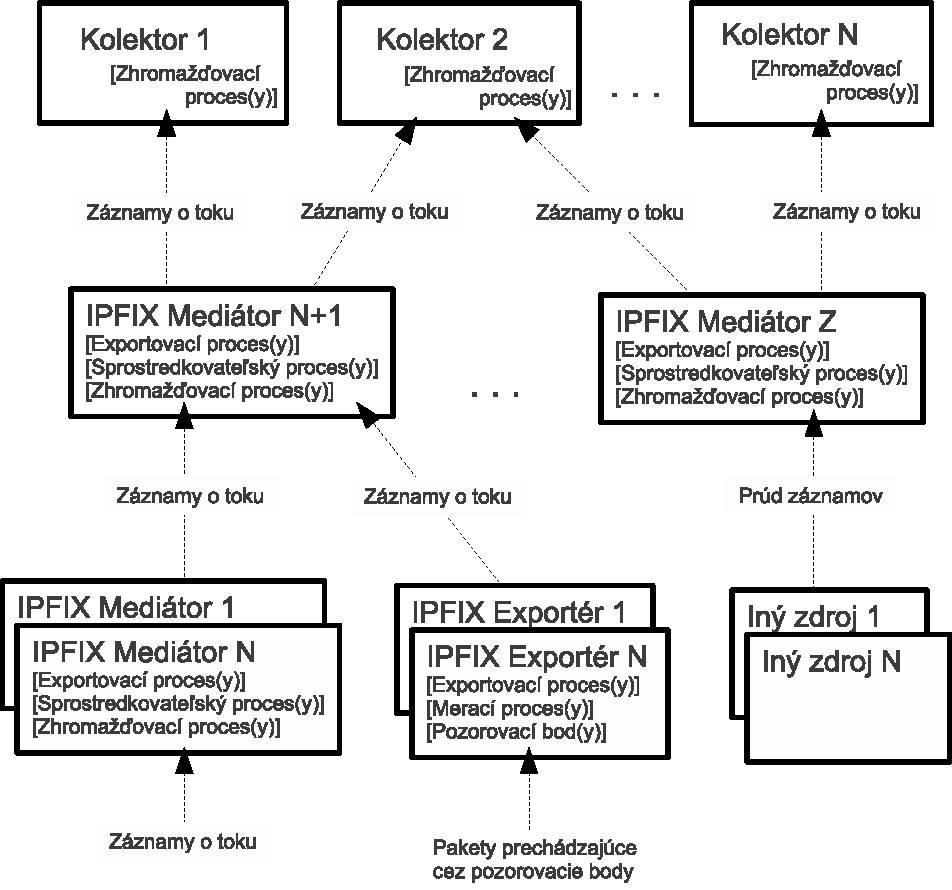
\includegraphics[width=0.9\textwidth]{mediation_reference_model}
\caption{Referen�n� model sprostredkovania spr�v v IPFIX}\label{o:mediation_reference_model}
\end{figure}

Anal�ze aplika�n�ho r�mca pre sprostredkovanie spr�v v IPFIX sa venuje RFC 6183 \citep{rfc6183}. 
Na Obr�zku \ref{o:mediation_reference_model} je zobrazen� referen�n� model sprostredkovania spr�v v IPFIX 
ako roz��renie referen�n�ho modelu IPFIX, pop�san�ho v \emph{Architecture for IP Flow Information Export} 
\citep{rfc5470}. T�to sch�ma zobrazuje mo�n� scen�re, ktor� m��u existova� v meracej architekt�re.



Funk�n� komponenty v r�mci ka�dej entity s� ohrani�en� z�tvorkami []. Medi�tor m��e prij�ma� 
z�znamy o toku od in�ch medi�torov a export�rov a pr�d z�znamov z in�ch zdrojov.
Za in� zdroje sa pova�uj� n�stroje in�ch protokolov, ako napr�klad NetFlow export�ry \citep{rfc3954}. 
Spracovane d�ta vo forme z�znamov o toku potom exportuje jedn�mu alebo viacer�m kolektorom a medi�torom.

\begin{figure}[ht!]
\centering
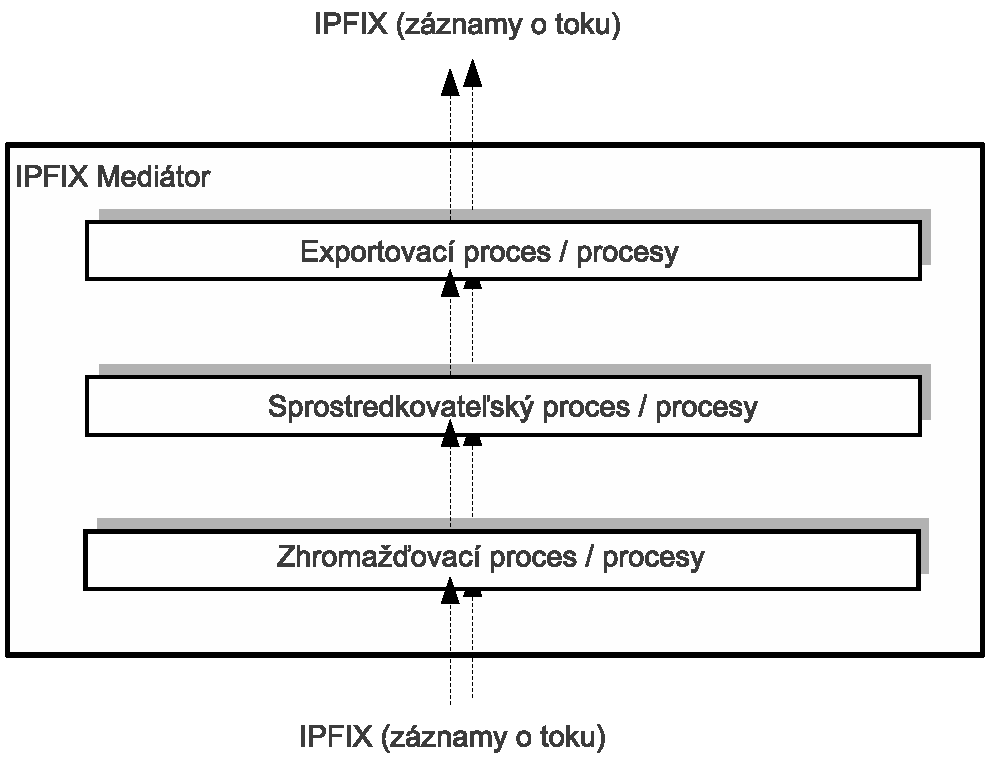
\includegraphics[width=0.7\textwidth]{mediator_component_model}
\caption{Zjednodu�en� model komponentov IPFIX Medi�tora}\label{o:mediator_component_model}
\end{figure}

Zjednodu�en� model komponentov IPFIX medi�tora je predstavuje Obr�zok \ref{o:mediator_component_model}. 
Medi�tor obsahuje jeden alebo viac sprostredkovate�sk�ch procesov, hierarchicky ulo�en�ch 
medzi jedn�m alebo viacer�mi exportovac�mi a zhroma��ovac�mi procesmi. Tento model sa t�ka 
najbe�nej�ieho pr�padu, kedy medi�tor prij�ma d�tov� z�znamy od export�ra, alebo in�ho medi�tora.

Sprostredkovate�sk� procesy s� k���ov�mi funk�n�mi blokmi sprostredkovania spr�v v IPFIX. Musia pokry� 
ka�d� pr�klad pou�itia sprostredkovania spr�v z kapitoly \ref{sec:mediator_examples}. 
Medi�tor je schopn� s��asne podporova� viac ako jeden sprostredkovate�sk� proces. 
\begin{itemize}
 \item \textbf{Paraleln� spracovanie} - Pr�d z�znamov je spracovan� viacer�mi sprostredkovate�sk�mi procesmi 
 paralelne. V tomto scen�ri, ka�d� sprostredkovate�sk� proces dost�va k�piu cel�ho pr�du z�znamov ako vstup.
 \item \textbf{S�riov� spracovanie} - Sprostredkovate�sk� procesy s� zapojene s�riovo. V�stupn� pr�d 
 z�znamov jedn�ho procesu je vstupn�m pr�dom nasleduj�ceho.
\end{itemize}

%--------------------------------------------

\clearpage

\section{Popis programu}

Jednotliv� �asti programu s� umiestnen� v~nasleduj�cich bal�koch:

\begin{itemize}
\item \verb|sk.tuke.cnl.bm.Mediator.collecting| - implement�cia zhroma��ovacieho procesu
\item \verb|sk.tuke.cnl.bm.Mediator.exporting| - implement�cia exportovacieho procesu
\item \verb|sk.tuke.cnl.bm.Mediator.IntermediateProcesses| - triedy tvoriace podporu pre sprostredkovate�sk� 
procesy. Hlavne triedy nov�ch modulov musia by� umiestnen� v tomto bal�ku!
\item \verb|sk.tuke.cnl.bm.Mediator.IPFIX| - triedy s~manu�lnou implement�ciou protokolu IPFIX
\item \verb|sk.tuke.cnl.bm.Mediator.exceptions| - vlastn� v�nimky aplik�cie
\item \verb|sk.tuke.cnl.bm.Mediator| - hlavn� triedy samotn�ho programu
\end{itemize}



\subsection{Popis rie�enia}


%V~prvom rade bolo potrebn� umo�ni� podporu viacer�ch z�znamov v~sade. Trieda NetXMLParser bola rozdelen� na dve samostatn� jednotky. Jednou je vl�kno UDPProcessor, ktor�ho �lohou je vybera� �daje z~PacketCache a �as� spracovania bole prep�san� do novej triedy IpfixParser. Parsovanie IPFIX spr�v bolo  zoptimalizovan� a upraven� do preh�adnej podoby. Celkov� probl�m bol rozdelen� na men�ie �lohy, ktor� s� realizovan� met�dami na parsovanie spr�vy, sady, a v�etk�ch druhov z�znamov. V~met�de sl��iacej na spracovanie sady bol pre ka�d� druh sady pridan� cyklus, ktor� vyber� z�znamy zo sady, a� k�m sa poz�cia v~buffri nedostane na koniec sady.
%
%Dek�dovanie d�t jednotliv�ch informa�n�ch elementov bolo presunut� do samostatnej  triedy. Podobne ako v~triede IpfixParser je volan� jedna met�da, ktor� na z�klade d�tov�ho typu presunie spracovanie na met�dy zaoberaj�ce sa danou skupinou d�tov�ch typov. �daje z~buffra pre d�tov� typ octetArray s� preveden� do podoby re�azce v~k�dovan� Base64 aby ich bolo mo�n� ulo�i� v~datab�ze. Bajt v~buffri pre d�tov� typ boolean je interpretovan� ako true pri hodnote 1 a ako false pri hodnote 0. V�etky ostatn� hodnoty znamenaj� chybu a je to ozn�men� volaj�cej met�de v�nimkou DataException. Okrem implement�cie dek�dovania d�tov�ho typu macAddres bola e�te opraven� interpret�cia d�tov�ch typov dateTimeMicroseconds a dateTimeNanoseconds. Ke�e sa tieto hodnoty musia zmesti� do �smich bajtov vo form�te NTP Timestamp a analyzuj�ce aplik�cie s� postaven� na technol�gii Java, ktor� nepozn� bezznamienkov� typy, je vhodn� ulo�i� tieto hodnoty v~nezmenenej podobe ako znamienkov� 64-bitov� ��slo (long). Po z�skan� ��sla 
%z~datab�zy je mo�n� jednoducho pou�i� triedu Timestamp z~kni�nice Apache Commons Net na jednoduch�iu pr�cu s~touto �asovou zn�mkou.
%
%Na podporu redukovan�ho k�dovania bola vytvoren� met�da handleReducedSizeEncoding(), ktor� zo skr�ten�ho informa�n�ho elementu vytvor� buffer plnej ve�kosti, ktor� je mo�n� be�n�m sp�sobom interpretova�. Pre bezznamienkov� ��sla sa do plnej ve�kosti z�ava doplnia nulov� bajty. Pre z�porn� znamienkov� ��sla sa doplnia bajty o~hodnote 255, aby sa zachovala hodnota ��sla. Redukovan� m��e by� aj d�tov� typ float64, a to pou�it�m polovi�n�ho po�tu bajtov. Vtedy sa d�ta interpretuj� ako float32.
%
%Organiz�ciou definovan� informa�n� elementy s� definovan� v~s�bore ipfixFields.xml. Aby sa uva�ovalo ��slo organiz�cie pre informa�n� elementy, musela by� doplnen� trieda IpfixElements o~mo�nos� evidencie informa�n�ch elementov nielen na z�klade ich identifik�tora, ale s��asne s~��slom organiz�cie (�tandardn� informa�n� elementy s� uva�ovan� s~��slom organiz�cie 0). Spolo�ne s~t�m v�etky met�dy sl��iace na pr�stup k~inform�ci�m o~informa�n�ch elementoch museli by� roz��ren� o~parameter ��sla organiz�cie.
%
%Variabiln� informa�n� elementy boli implementovan� v~triede IpfixParser. Pri v�bere informa�n�ho elementu, ktor�ho ve�kos� je v~z�zname �abl�ny definovan� ako 65535 je vybrat� prv� bajt z~d�tovej �asti na aktu�lnej poz�cii. Ak je tento bajt men�� ako 255, je vybran�ch to�ko bajtov z~buffra, ko�ko tento bajt uv�dza. Ak m� bajt hodnotu 255, d�ka je z�skan� z~�al��ch dvoch bajtov.
%
%S��as�ou zmien v~parseri je detekcia po�koden�ch spr�v. Ak je skuto�n� ve�kos� spr�vy in� ako sa uv�dza v~hlavi�ke, ide o~chybu. Pri ka�dej chybe je vyhoden� v�nimka DataFormatException. Chyba je indikovan� aj ke� je po�et zost�vaj�cich bajtov v~buffri men�� ako ve�kos� sady. Pri v�bere �dajov z~d�tov�ho z�znamu alebo z�znamu �abl�ny sa testuje n�raz na prav� hranicu sady. V~pr�pade jej dosiahnutia sa tie� ohl�si chyba.
%
%Na pridanie podpory expir�cie �abl�n musela sa do z�znamu �abl�ny prida� polo�ka �asu pr�chod �abl�ny. Cache bola spreh�adnen� a pred parsovan�m
%d�tov�ho z�znamu je overovan� platos� �abl�ny. V~pr�pade ak je neplatn�, d�tov� sada sa presko��. Ka�d�ch 10 min�t sa sp���a �istiace vl�kno, aby vymazalo expirovan� �abl�ny a zabr�nilo tak zapl�ovaniu pam�te JXColl.
%Transportn� protokoly TCP a SCTP pou��vaj� vlastn� cache na uschovanie �abl�n s~platnos�ou len pre konkr�tne pripojenie, resp. asoci�ciu.
%Umo��en� bola podpora pre zru�enie �abl�n pomocou Template Withdrawal spr�v. V~pr�pade, ak export�r po�le u� kolektorom evidovan� �abl�nu, alebo ak ru�� neexistuj�cu �abl�nu, spojenie, resp. asoci�cia sa preru��. 
%
%Protokoly TCP a SCTP vyu��vaj� na ka�d� pripojenie samostatn� vl�kno. Obidva protokoly po��vaj� na nakonfigurovanom porte a po�et pripojen�, resp. asoci�ci� je ohrani�en� nastaven�m v~konfigura�nom s�bore. Na podporu protokolu SCTP bolo potrebn� prejs� na nov�iu verziu Javy 1.7.




\clearpage
\section{Popis tried, �lensk�ch premenn�ch a~met�d}

Ke�e niektor� triedy Medi�tora s� kv�li jednotnosti rie�en� v r�mci v�skumnej skupiny MONICA toto�n� 
s triedami nastroja JXColl, v~nasleduj�cich �astiach bud� uveden� len tie, ktor� sa tykaj� v�hradne 
Medi�tora. Popis ostatn�ch tried a~met�d je uveden� v~syst�movej pr�ru�ke programu 
JXColl \citep{jxcoll_sp}.  

% ----------HLAVN� BAL�K --------------------------------------

\subsection{Bal�k sk.tuke.cnl.bm.Mediator}

\subsubsection{Trieda Default}
Trieda predstavuje rozhranie obsahuj�ce v�chodiskov� hodnoty konfigura�n�ho s�boru. Neobsahuje kon�truktor
ani �iadne met�dy, iba verejne pr�stupn� statick� kon�tanty.



\subsubsection{Trieda DropsCounter}
Sl��i na v�po�et �tatistiky zahoden�ch ent�t. Pod entitou sa myslia z�znamy o tokoch, d�tov� z�znamy, 
alebo IPFIX pakety. Obsahuje len statick� met�dy.

\bigskip
\textbf{Met�dy} 

\textit{public static void \textbf{inputBufferDropsUP}()}

Zvy�uje po�et str�t sp�soben�ch preplnen�m vstupn�ho buffera sprostredkovate�sk�ch procesov o jeden. \\
\textbf{Parametre:} \\
\emph{String} processName - meno procesu


\textit{public static void \textbf{exportCacheDropsUP}()}

Zvy�uje po�et str�t sp�soben�ch \verb|ExportCache| o jeden.\\


\textit{public static void \textbf{encodingDropsUp}()}

Zvy�uje po�et str�t sp�soben�ch chybou pri k�dovan� o jeden.\\


\textit{public static void \textbf{decodingDropsUp}()}

Zvy�uje po�et str�t sp�soben�ch chybou pri dek�dovan� o jeden.\\


\textit{public static void \textbf{packetDropsUp}()}

Zvy�uje po�et IPFIX paketov zahoden�ch UDP serverom o jeden.\\


\textit{public static void \textbf{printStats}()}

Vyp��e �tatistiku v�etk�ch zahoden�ch ent�t.



\subsubsection{Trieda FlowRecordDispatcher}
�lohou tejto triedy je na z�klade konfigura�n�ho s�boru distribuova� prijat� z�znamy o toku 
sprostredkovate�sk�m procesom (s�riovo alebo paralelne) a exportovaciemu procesu. Distrib�cia prebieha
v s�lade s IPFIX Mediator Framework (RFC 6183). T�to trieda je implementovan� pod�a n�vrhov�ho vzoru 
\emph{Singleton}.

\bigskip
\textbf{Met�dy} 

\textit{public static FlowRecordDispatcher \textbf{getInstance}()}

Implementuje vzor \emph{Singleton}. Vytvor� a vr�ti jedine�n� in�tanciu v pr�pade �e neexistuje, v 
opa�nom pr�pade ju iba vr�ti. \\
\textbf{N�vratov� hodnota:} \\
Jedine�n� objekt typu \verb|FlowRecordDispatcher|.\\


\textit{public synchronized void \textbf{dispatchFlowRecord}(IPFIXFlowRecord flowRecord, String inputProcess)}

Posiela prijat� z�znamy o tokoch pr�slu�n�m sprostredkovate�sk�m procesom, alebo exportovaciemu procesu 
pod�a konfigur�cie. Najprv z�ska zoznam prij�mate�ov toku na z�klade mena p�vodcu. Ak je zoznam pr�zdny - 
z�znam o toku je 
ur�en� na export, preto ho zap��e do \verb|ExportCache|. Ak zoznam nie je pr�zdny, z�ska si in�tancie 
prij�mate�ov toku a z�znam im zap��e do vstupn�ho buffera. T�to met�da je synchronizovan�, lebo je
pr�stupn� viacer�m vl�knam. \\
\textbf{Parametre:} \\
\emph{IPFIXFlowRecord} flowRecord - z�znam o toku, ktor� sa m� distribuova� �alej \\
\emph{String} inputProcess - meno p�vodcu z�znamu o toku.\\

\textit{private void \textbf{fillInputBuffer}(AIntermediateProcess process, IPFIXFlowRecord flowRecord)}

Met�da, ktor� zapisuje z�znamy o tokoch do vstupn�ho buffera sprostredkovate�sk�ch procesov. V pr�pade
ne�spechu sa zv��i po��tadlo v \verb|DropsCounter| a vyp��e error. \\
\textbf{Parametre:} \\
\emph{AIntermediateProcess} process - in�tancia sprostredkovate�sk�ho procesu. \\
\emph{IPFIXFlowRecord} flowRecord - z�znam o toku, ktor� sa m� zap�sa�.\\

\textit{private ArrayList$<$String$>$ \textbf{getReceiversList}(String inputDevice)}

Z�skava zoznam pr�jemcov z�znamu o toku od zadan�ho p�vodcu toku. \\
\textbf{Parametre:} \\
\emph{String} inputDevice - p�vodca z�znamu o toku \\
\textbf{N�vratov� hodnota:} \\
Zoznam pr�jemcov toku, typ \verb|ArrayList|.



\subsubsection{Trieda IPLoader}
Trieda je zodpovedn� za dynamick� na��tavanie sprostredkovate�sk�ch procesov definovan�ch v konfigura�nom
s�bore. Implementuje n�vrhov� vzor \emph{Singleton}.

\bigskip
\textbf{Met�dy} 

\textit{public static IPLoader \textbf{getInstance}()}

Implementuje vzor \emph{Singleton}. Vytvor� a vr�ti jedine�n� in�tanciu v pr�pade �e neexistuje, v opa�nom pr�pade 
ju iba vr�ti.\\


\textit{public void \textbf{loadProcesses}()}

Hlavn� met�da triedy, dynamicky na��tava sprostredkovate�sk� moduly definovan� v konfigura�nom s�bore. 
Najprv z�ska syst�mov� \emph{classLoader}. V cykle prech�dza zoznam sprostredkovate�sk�ch modulov. 
Ka�d� re�azec obsahuj�ci meno prevedie na bin�rne meno (meno triedy vr�tane bal��kov)  a pomocou 
classLoader-a z�ska jeho \verb|Class| objekt. Na z�klade tohto objektu z�ska jedine�n� in�tanciu 
modulu a ke�e sa jedn� o vl�kno, spust� ho tak, �e zavol� jeho met�du \verb|start()|. \\
\textbf{H�d�e:} \\
\verb|IPLoaderException| - V pr�pade akejko�vek chyby, ktor� m��e nasta� pri vykon�van� met�dy. Chyby, ktor� 
s� zachyt�van� s� typov:
\begin{itemize}
 \item \verb|SecurityException|
 \item \verb|ClassNotFoundException|
 \item \verb|IllegalAccessException|
 \item \verb|NoSuchMethodException|
 \item \verb|InvocationTargetException|
\end{itemize}



\subsubsection{Trieda Mediator}
�lohou hlavnej triedy Medi�tora je postupne spusti� v�etky vl�kna a procesy potrebn� pre beh programu.
Najprv sa pre��taj� a spracuj� argumenty pr�kazov�ho riadku. Program vie rozpozn�va� dva druhy 
argumentov. Prv�m je cesta ku konfigura�n�mu s�boru. Ak nie je zadan�, pou��va sa v�chodiskov� 
konfigura�n� s�bor. Druh�m argumentom m��e by� zadan� mo�nos� \verb|--logtofile|. Vtedy s� v�etky 
logovacie v�stupy presmerovan� zo �tandardn�ho v�stupu do s�boru.

Potom ako program na��ta v�etky nastavenia z konfigura�n�ho s�boru, spust� v�etky svoje moduly - 
sprostredkovate�sk� procesy pomocou triedy \verb|IPLoader|. Nasleduje spustenie vl�kna, ktor� prij�ma 
IPFIX pakety prostredn�ctvom protokolu UDP a vl�kna, ktor� ich spracov�va. Hovor�me o \verb|UDPServer| 
a \verb|UDPProcessor|. Nakoniec je spusten� exportovacie vl�kno - \verb|UDPExporter|. Kedyko�vek ke� 
nastane chyba je Medi�tor korektne ukon�en� a to tak, �e uvoln� v�etku pam� a zastav� be�iace vl�kna. 
Rovnako je Medi�tor zastaven� po stla�en� kombin�cie kl�ves \verb|Ctrl+c|.

\bigskip
\textbf{Met�dy} 

\textit{public static void \textbf{main}(String[] args)}

Hlavn� met�da triedy. \\
\textbf{Parametre:} \\
\emph{String[]} args - argumenty pr�kazov�ho riadku.\\


\emph{public static void \textbf{stopMediator}()}

Met�da, ktor� korektne ukon�uje beh programu. Zastav� v�etky spusten� vl�kna a uvo�n� v�etky druhy pam�te.\\

\clearpage
\emph{public static void \textbf{interruptThread}()}

Preru�� vykon�vanie vl�kna. \\
\textbf{Parametre:} \\
\emph{Thread} thread - objekt vl�kna, ktor� sa m� zastavi�.\\


\emph{private static void \textbf{loggingToFile}()}

Met�da, ktor� vykon�va logovanie do s�boru namiesto �tandardn�ho v�stupu.



\subsubsection{Trieda Support}
Podporn� trieda, ktor� obsahuje pomocn� met�dy potrebn� pri de(k�dovan�) a pri valid�cii form�tu d�t. 
Uv�dzam iba vlastn� met�dy.

\bigskip
\textbf{Met�dy} 


\emph{public static byte[] \textbf{byteToByteArray}(byte x)}

Konvertuje primit�vny typ \emph{byte} na pole bytov v usporiadan� bytov Big Endian. \\
\textbf{Parametre:} \\
\emph{byte} x - hodnota, ktor� sa m� zak�dova�. \\
\textbf{N�vratov� hodnota:} \\
Pole bytov, typ \emph{byte[]}. \\


\emph{public static byte[] \textbf{shortToByteArray}(short x)}

Konvertuje primit�vny typ \emph{short} na pole bytov v usporiadan� bytov Big Endian. \\
\textbf{Parametre:} \\
\emph{short} x - hodnota, ktor� sa m� zak�dova�. \\
\textbf{N�vratov� hodnota:} \\
Pole bytov, typ \emph{byte[]}. \\


\emph{public static byte[] \textbf{intToByteArray}(int x)}

Konvertuje primit�vny typ \emph{int} na pole bytov v usporiadan� bytov Big Endian. \\
\textbf{Parametre:} \\
\emph{int} x - hodnota, ktor� sa m� zak�dova�. \\
\textbf{N�vratov� hodnota:} \\
Pole bytov, typ \emph{byte[]}. \\


\emph{public static byte[] \textbf{longToByteArray}(long x)}

Konvertuje primit�vny typ \emph{long} na pole bytov v usporiadan� bytov Big Endian. \\
\textbf{Parametre:} \\
\emph{long} x - hodnota, ktor� sa m� zak�dova�. \\
\textbf{N�vratov� hodnota:} \\
Pole bytov, typ \emph{byte[]}. \\


\emph{public static byte[] \textbf{floatToByteArray}(float x)}

Konvertuje primit�vny typ \emph{float} na pole bytov v usporiadan� bytov Big Endian. \\
\textbf{Parametre:} \\
\emph{float} x - hodnota, ktor� sa m� zak�dova�. \\
\textbf{N�vratov� hodnota:} \\
Pole bytov, typ \emph{byte[]}. \\


\emph{public static byte[] \textbf{doubleToByteArray}(double x)}

Konvertuje primit�vny typ \emph{double} na pole bytov v usporiadan� bytov Big Endian. \\
\textbf{Parametre:} \\
\emph{double} x - hodnota, ktor� sa m� zak�dova�. \\
\textbf{N�vratov� hodnota:} \\
Pole bytov, typ \emph{byte[]}. \\


\emph{public static boolean \textbf{validateMAC}(String macAddress)}

Validuje form�t MAC adresy. \\
\textbf{Parametre:} \\
\emph{String} macAddress - adresa, ktorej form�t sa m� overi�. \\
\textbf{N�vratov� hodnota:} \\
\emph{true} - v pr�pade, �e je adresa v spr�vnom form�te.\\
\emph{false} - opa�ne.





% ----------BAL�K IPFIX --------------------------------------

\subsection{Bal�k sk.tuke.cnl.bm.Mediator.IPFIX}

\subsubsection{Trieda IPFIXEncoder}
Trieda so statick�mi met�dami sl��iacimi na zak�dovanie re�azcovej reprezent�cie hodn�t informa�n�ch
elementov na abstraktne d�tov� typy pod�a RFC 5101 a RFC 5102. Je presn�m opakom triedy \verb|IPFIXDecoder|.


\bigskip
{\bfseries Met�dy}


\textit{public static byte[] \textbf{encode}(String dataType, String value)}

Zak�duje hodnotu d�tov�ho typu do po�a bytov pod�a �pecifik�cie IPFIX.
Priamo nevykon�va zak�dovanie, vol� konkr�tne met�dy pod�a kateg�rie d�tov�ho typu.\\
{\bfseries Parametre:}\\
\emph{String} dataType - re�azec definuj�ci d�tov� typ obsiahnut� v~bufferi.\\
\emph{String} value - samotn� d�ta, ktor� s� predmetom zak�dovania\\
{\bfseries N�vratov� hodnota:} \\
Pole bytov reprezentuj�ce interpretovan� re�azcov� hodnotu na z�klade predan�ho typu. \\
{\bfseries H�d�e:} \\
\verb|UnsupportedDataException| - Ak d�tov� typ nie je podporovan�\\
\verb|OutOfBoundsException| - Ak je hodnota mimo povolen�ho rozsahu\\
\verb|UnknownHostException| - Ak program nevie rozpozna� host, alebo IP adresu \\
\verb|DataException| - Ak je chyba v form�te k�dovanej hodnoty vzh�adom na d�tov� typ\\



\textit{public static byte[] \textbf{encodeUnsignedIntegralType}(String dataType, String value)}

Zak�duje celo��seln� bezznamiekov� d�tov� typy unsigned8, unsigned16, unsigned32, unsigned64 a unsigned128. \\
{\bfseries Parametre:}\\
\emph{String} dataType - re�azec definuj�ci d�tov� typ obsiahnut� v~bufferi.\\
\emph{String} value - samotn� d�ta, ktor� s� predmetom zak�dovania\\
{\bfseries N�vratov� hodnota:} \\
Pole bytov reprezentuj�ce interpretovan� re�azcov� hodnotu na z�klade predan�ho typu. \\
{\bfseries H�d�e:} \\
\verb|UnsupportedDataException| - Ak d�tov� typ nie je podporovan�\\
\verb|NumberFormatException| - Ak je chyba v form�te k�dovanej hodnoty vzh�adom na d�tov� typ\\
\verb|OutOfBoundsException| - Ak je hodnota mimo povolen�ho rozsahu\\



\textit{public static byte[] \textbf{encodeSignedIntegralType}(String dataType, String value)}

Zak�duje celo��seln� znamienkov� d�tov� typy signed8, signed16, signed32 a signed64. \\
{\bfseries Parametre:}\\
\emph{String} dataType - re�azec definuj�ci d�tov� typ obsiahnut� v~bufferi.\\
\emph{String} value - samotn� d�ta, ktor� s� predmetom zak�dovania\\
{\bfseries N�vratov� hodnota:} \\
Pole bytov reprezentuj�ce interpretovan� re�azcov� hodnotu na z�klade predan�ho typu. \\
{\bfseries H�d�e:} \\
\verb|UnsupportedDataException| - Ak d�tov� typ nie je podporovan�\\
\verb|NumberFormatException| - Ak je chyba v form�te k�dovanej hodnoty vzh�adom na d�tov� typ\\




\textit{public static byte[] \textbf{encodeFloatType}(String dataType, String value)}

Zak�duje desatinn� d�tov� typy float32 a float64. \\
{\bfseries Parametre:}\\
\emph{String} dataType - re�azec definuj�ci d�tov� typ obsiahnut� v~bufferi.\\
\emph{String} value - samotn� d�ta, ktor� s� predmetom zak�dovania\\
{\bfseries N�vratov� hodnota:} \\
Pole bytov reprezentuj�ce interpretovan� re�azcov� hodnotu na z�klade predan�ho typu. \\
{\bfseries H�d�e:} \\
\verb|UnsupportedDataException| - Ak d�tov� typ nie je podporovan�\\
\verb|NumberFormatException| - Ak je chyba v form�te k�dovanej hodnoty vzh�adom na d�tov� typ\\




\textit{public static byte[] \textbf{encodeAddressType}(String dataType, String value)}

Zak�duje d�tov� typy obsahuj�ce adresy: ipv4Address, ipv6Address a macAddress. \\
{\bfseries Parametre:}\\
\emph{String} dataType - re�azec definuj�ci d�tov� typ obsiahnut� v~bufferi.\\
\emph{String} value - samotn� d�ta, ktor� s� predmetom zak�dovania\\
{\bfseries N�vratov� hodnota:} \\
Pole bytov reprezentuj�ce interpretovan� re�azcov� hodnotu na z�klade predan�ho typu. \\
{\bfseries H�d�e:}\\
\verb|UnsupportedDataException| - Ak d�tov� typ nie je podporovan�\\
\verb|UnknownHostException| - Ak program nevie rozpozna� host, alebo IP adresu \\
\verb|DataException| - Ak je chyba v form�te k�dovanej hodnoty vzh�adom na d�tov� typ\\




\textit{public static byte[] \textbf{encodeBooleanType}(String value)}

Zak�duje boolean reprezentuj�ci pravdivostn� hodnotu.\\
{\bfseries N�vratov� hodnota:}\\
Pole bytov reprezentuj�ci pravdivostn� hodnotu, "true" alebo "false". \\
{\bfseries H�d�e:} \\
\verb|OutOfBoundsException| - Ak je hodnota mimo povolen�ho rozsahu\\



\textit{public static byte[] \textbf{encodeStringType}(String value)}

Zak�duje re�azec v k�dovan� UTF-8 do pole bytov.\\
{\bfseries N�vratov� hodnota:}\\
Pole bytov re�azca v~k�dovan� UTF-8.\\



\textit{public static byte[] \textbf{encodeOctetArrayType}(String value)}

Re�azec v k�du Base64 prevedie na pole bytov.\\
{\bfseries N�vratov� hodnota:}\\
Pole bytov predstavuj�ce bin�rne d�ta zak�dovan� v~Base64. \\



\textit{public static byte[] \textbf{encodeDateTimeType}(String dataType, String value)}

Zak�duje d�tov� typy �asov�ch zn�mok: dateTimeSeconds, dateTimeMilliseconds, dateTimeMicroseconds a 
dateTimeNanoseconds do po�a bytov. \\
{\bfseries Parametre:}\\
\emph{String} dataType - re�azec definuj�ci d�tov� typ obsiahnut� v~bufferi.\\
\emph{String} value - samotn� d�ta, ktor� s� predmetom zak�dovania\\
{\bfseries N�vratov� hodnota:}\\
Pole bytov reprezentuj�ce interpretovan� hodnotu re�azca na z�klade predan�ho typu.
D�tov� typy dateTimeSeconds a dateTimeMilliseconds predstavuj� po�et sek�nd, resp. milisek�nd od Unix 
epochy (00:00 1.1.1970 UTC).
D�tov� typy dateTimeMicroseconds a dateTimeNanoseconds s� zak�dovan� vo form�te �asovej zn�mky NTP 
Timestamp.\\
{\bfseries H�d�e:}\\
\verb|UnsupportedDataException| - Ak d�tov� typ nie je podporovan�\\
\verb|NumberFormatException| - Ak je chyba v form�te k�dovanej hodnoty vzh�adom na d�tov� typ\\
\verb|OutOfBoundsException| - Ak je hodnota mimo povolen�ho rozsahu\\



\textit{public static void \textbf{checkStringNumbersRange}(String min, String max, String value, String dataType)}

Over�, �i ��seln� hodnota v re�azci spad� do rozsahu dan�ho d�tov�m typom. \\
{\bfseries Parametre:}\\
\emph{String} min - doln� hranica rozsahu \\
\emph{String} max - horn� hranica rozsahu\\
\emph{String} value - hodnota, ktor� sa m� overi�\\
\emph{String} dataType - d�tov� typ hodnoty\\
{\bfseries H�d�e:}\\
\verb|OutOfBoundsException| - Ak je hodnota mimo povolen�ho rozsahu




\subsubsection{Trieda IPFIXFlowRecord}
T�to trieda je reprezent�ciou IPFIX Flow record-u, teda z�znamu o toku.

\bigskip
\textbf{Kon�truktor} 

\textit{public \textbf{IPFIXFlowRecord}(IPFIXTemplateRecord referencedTemplate, 
ArrayList $<$IPFIXDataRecord$>$ dataRecords, IPFIXMessage.IPFIXMessageHeader messageHeader)}

Kon�truktor prostredn�ctvom predan�ch parametrov inicializuje �lensk� premenn�.\\
\textbf{Parametre:}\\
\emph{IPFIXTemplateRecord} referencedTemplate - �abl�na patriaca d�tov�m z�znamom\\
\emph{ArrayList$<$IPFIXDataRecord$>$} dataRecords - pole d�tov�ch z�znamov\\
\emph{IPFIXMessage.IPFIXMessageHeader} messageHeader - hlavi�ka IPFIX spr�vy, ktor� obsahovala tento
z�znam o toku


\emph{public \textbf{IPFIXFlowRecord}()}

Bezparametrick� kon�truktor. Iba inicializuje pr�zdne pole d�tov�ch z�znamov. \\


\textbf{Met�dy:}\\
Met�dy, ktor� tu nie s� spomenut�, s� klasick� gettery a settery.



\emph{public int \textbf{getReferencedTemplateID}()}

{\bfseries N�vratov� hodnota:}\\
Vracia ID �abl�ny z IPFIX spr�vy, ktor� obsahovala tento z�znam o toku.\\



\clearpage
\emph{public void \textbf{addDataRecord}(IPFIXDataRecord dataRecord)}

Prid� d�tov� z�znam do po�a d�tov�ch z�znamom flow record-u.\\
\textbf{Parametre:}\\
\emph{IPFIXDataRecord} dataRecord - d�tov� z�znam, ktor� sa prirad� z�znamu o toku.



\subsubsection{Trieda IPFIXMessageHeader}
Trieda reprezentuj�ca hlavi�ku IPFIX spr�vy. Implementuje n�vrhov� vzor Singleton.

\bigskip
\textbf{Metody:}\\
Met�dy, ktor� tu nie s� spomenut�, s� klasick� gettery a settery.

\emph{public static IPFIXMessageHeader \textbf{getInstance}()}

{\bfseries N�vratov� hodnota:}\\
Vracia jedine�n� in�tanciu objektu.





% ----------BAL�K INTERMEDIATE PROCESS ----------------------------------

\subsection{Bal�k sk.tuke.cnl.bm.Mediator.IntermediateProcesses}


Diagram tried rozhrania pre sprostredkovate�sk� procesy, vr�tane triedy \verb|ExampleProcess| je zn�zornen�
na obr�zku \ref{o:intermediate_class}.

\begin{figure}[ht!]
\centering
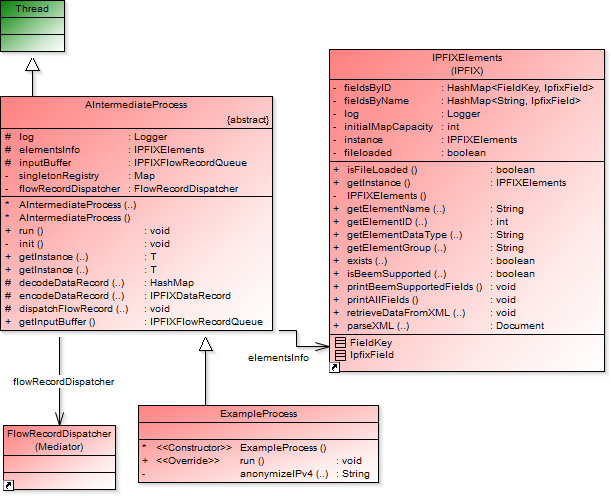
\includegraphics[width=1.0\textwidth]{intermediate_class}
\caption{Diagram tried rozhrania pre sprostredkovate�sk� procesy}\label{o:intermediate_class}
\end{figure}



\subsubsection{Trieda AIntermediateProcess}
Abstraktn� trieda, poskytuje v�chodiskov� met�dy sprostredkovate�sk�m procesom a tvori ak�si
rozhranie medzi modulmi a aplika�n�m r�mcom. Ded� od triedy \verb|Thread|.\\
\\
\\

\bigskip
\textbf{Kon�truktor} 

\emph{\textbf{AIntermediateProcess}(String childName)}

Nastav� meno procesu, pod�a prijat�ho parametra. Inicializuje vstupn� buffer a z�ska jedine�n� in�tanciu
triedy \verb|IPFIXElements|.\\
\textbf{Parametre:}\\
\emph{String} childName - meno triedy potomka

\emph{\textbf{AIntermediateProcess}()}

Bezparametrick� kon�truktor. Inicializuje vstupn� buffer a z�ska jedine�n� in�tanciu
triedy \verb|IPFIXElements|.\\


\textbf{Metody:}\\

\emph{public static final synchronized $<$T extends AIntermediateProcess$>$ T \textbf{getInstance} (Class clazz)}

Toto rie�enie je hybridom viacer�ch pr�stupov, ktor� sa diskutuj� na Internete, no vych�dza z 
n�vrhov�ho vzoru \emph{Factory method}. V�sledkom je abstraktn� trieda, sl��iaca ako tov�re� na 
podtriedy t�m, �e vol� jej statick� met�du \emph{getInstance(Class clazz)}. 
Ak s� splnen� podmienky, �e konkr�tna trieda, napr. \verb|SelectionProcess| je definovan� v rovnakom 
bal��ku ako \verb|AIntermediateProcess| a ich kon�truktory nemaj� explicitne nastaven� pr�stup 
(predvolen�m pr�stupom je \uv{priv�tny v r�mci bal��ka}), tak 
jedin�m sp�sobom ako z�ska� in�tanciu podtriedy mimo bal��ka je cez kon�trukciu:
\begin{verbatim}
 SelectionProcess instance = 
 AIntermediateProcess.getInstance(SelectionProcess.class);
\end{verbatim}
Dalo by sa vy��ta�, �e vytv�ranie in�tanci� pou��va reflexiu, ktor� je pomal�. Av�ak, ke�e vytv�rame 
Singletony, volanie \emph{newInstance()} sa vykon� pre ka�d� modul prav� raz. \\
\textbf{Parametre:}\\
\emph{Class} clazz = class objekt po�adovanej triedy \\
\textbf{N�vratov� hodnota:}\\
Objekt typu T, pri�om T dedi od \verb|AIntermediateProcess|.



\emph{public static final synchronized $<$T extends AIntermediateProcess$>$ T \textbf{getInstance} (String processName)}
   
Aby bolo mo�n� z�skava� in�tancie modulov aj na z�klade mena triedy a nie len cez class objekty, vytvoril 
som t�to met�du. Premenn� \emph{processName} prevedie na bin�rne meno procesu, pod�a �pecifik�cie jazyka 
Java, teda n�zov triedy vr�tane bal��kov, napr. 
\verb|sk.tuke.cnl.Mediator.SelectionProcess|.
T�to met�da na��ta \emph{class} objekt sprostredkovate�sk�ho procesu cez syst�mov� class loader,
tak ako to bolo vy��ie spom�nan�. Potom zavol� p�vodn� met�du \emph{getInstance(Class clazz)} a 
vr�ti in�tanciu procesu.\\
\textbf{Parametre:}\\
\emph{String} processName = meno po�adovanej triedy \\
\textbf{N�vratov� hodnota:}\\
Objekt typu T, pri�om T dedi od \verb|AIntermediateProcess|.\\




\emph{protected final HashMap \textbf{decodeDataRecord}(IPFIXTemplateRecord template, IPFIXDataRecord dataRecord)}

Pri prvom prechode funkciou sa generuje pam�ov� z�znam o informa�n�ch elementoch (ie) z XML s�boru. 
Vytiahnu sa inform�cie o ie, ktor� sa nach�dzaj� v �abl�ne, dek�duj� sa ich d�tov� typy a pr�slu�nos� k 
skupine.\\
\textbf{Parametre:}\\
\emph{IPFIXTemplateRecord} template - �abl�na d�t\\
\emph{IPFIXDataRecord} dataRecord - d�tov� z�znam\\
\textbf{N�vratov� hodnota:}\\
Dek�dovan� d�ta ako objekt typu \verb|HashMap|.\\


\emph{protected final IPFIXDataRecord \textbf{encodeDataRecord}(IPFIXTemplateRecord template, 
HashMap$<$String, String$>$ dataMap)}

Zak�duje v�etky hodnoty z hashmapy obsahuj�cej hodnoty informa�n�ch elementov pod�a �abl�ny do d�tov�ho 
z�znamu. \\
\textbf{Parametre:}\\
\emph{IPFIXTemplateRecord} template - �abl�na d�t \\
\emph{HashMap$<$String, String$>$} dataMap - hodnoty informa�n�ch elementov v hashmape, ktor� sa m� zak�dova�\\
\textbf{N�vratov� hodnota:}\\
Vracia objekt d�tov�ho z�znamu -  \verb|IPFIXDataRecord|.\\
\textbf{H�d�e:}\\
\verb|EncodingException| - Ak nastane chyba pri k�dovan�.\\



\emph{protected final void \textbf{dispatchFlowRecord}(IPFIXFlowRecord flowRecord, String inputProcess)}

Vytv�ra rozhranie pre pr�stup k met�de aplika�n�ho r�mca.\\
\textbf{Parametre:}\\
\emph{IPFIXFlowRecord} flowRecord - z�znam o toku, ktor� sa m� posun�� �alej \\
\emph{String} inputProcess - p�vodca z�znamu o toku 



\subsubsection{Trieda ExampleProcess}

T�to trieda je vzorov�m rie�en�m jednoduch�ho sprostredkovate�sk�ho procesu, vykon�vaj�ceho 
anonymiz�ciu. ��elom triedy je pomoc �al�ej gener�cii rie�ite�ov.

\bigskip
\textbf{Kon�truktor} 

\emph{\textbf{ExampleProcess}()}

Vola rodi�ovsk� kon�truktor a pred�va mu svoje meno ako parameter.\\

\textbf{Metody:}\\
\emph{public void \textbf{run}()}

Hlavn� met�da vl�kna. V cykle �ak� na z�znamy o tokoch vo svojom vstupnom bufferi \emph{(inputBuffer)} a 
postupne ich odtia� ��ta a odstra�uje. Nazvime ich 
\emph{vstupne z�znamy}. Vstupn� buffer jej nap��a trieda \verb|FlowRecordDispatcher|. Po pre��tan� 
vstupn�ho z�znamu vytvor� a inicializuje \emph{v�stupn� z�znam}. N�sledne prech�dza v�etky d�tov� z�znamy
vstupn�ho z�znamu, dek�duje ich, anonymizuje zdrojov� a cie�ov� IP adresu a naspa� zak�duje. Ak v�etko 
prebehlo bez probl�mov, tak d�tov� z�znam prirad� v�stupn�mu z�znamu. Napokon v�stupn� z�znam o toku 
posunie distrib�torovi z�znamov, ktor� ho bude prepo�le 
nasleduj�cemu sprostredkovate�sk�mu procesu, alebo priprav� na export. \\


\emph{private String \textbf{anonymizeIPv4}(String address)}

Met�da na ve�mi jednoduch� anonymiz�ciu IP adresy, ��slo v poslednom oktete zmen� na 0.\\
\textbf{Parametre:}\\
\emph{String} address - IP adresa, ktor� sa anonymizova� \\
\textbf{N�vratov� hodnota:}\\
Anonymizovan� IP adresa, vr�ten� ako re�azec.



\subsubsection{Trieda IPInputBuffer}

Reprezentuje vstupn� buffer sprostredkovate�sk�ch modulov. T�to trieda je cache pre z�znamy o tokoch. 
Jej pou�itie je kritick� vo vysokor�chlostn�ch sie�ach, preto�e udr�iava elementy a t�m p�dom m��e 
vyrovn�va� n�razov� n�por. Je synchronizovan� a jej implement�cia je FIFO front typu \verb|ArrayBlockingQueue|.\\

\textbf{Met�dy:}

\emph{public boolean \textbf{write}(IPFIXFlowRecord flowRecord)}

Zapisuje z�znamy o tokoch do frontu. Ak je front pln�, z�znam sa zahadzuje.\\
\textbf{Parametre:}\\
\emph{IPFIXFlowRecord} flowRecord - z�znam o toku\\
\textbf{N�vratov� hodnota:}\\
Pravdivostn� hodnota pod�a toho, �i z�znam bol, alebo nebol zap�san� do cache.\\


\emph{public void \textbf{write}(IPFIXTemplateRecord template, ArrayList$<$IPFIXDataRecord$>$ dataRecords, IPFIXMessage.IPFIXMessageHeader messageHeader)}

Met�da obal� prijat� parametre do objektu triedy \verb|IPFIXFlowRecord| a zavol� predch�dzaj�cu met�du.\\
\textbf{Parametre:}\\
\emph{IPFIXTemplateRecord} template - �abl�na\\
\emph{ArrayList$<$IPFIXDataRecord$>$} dataRecords - pole d�tov�ch z�znamov\\
\emph{IPFIXMessage.IPFIXMessageHeader} messageHeader - hlavi�ka IPFIX spr�vy, z ktorej tento z�znam o toku 
poch�dza\\



\emph{public IPFIXFlowRecord \textbf{read}()}

Pre��ta a zma�e vrchol frontu. Ak je front pr�zdny �ak� dokia� sa tam nejak� element neprid�.\\
\textbf{N�vratov� hodnota:}\\
Objekt triedy \verb|IPFIXFlowRecord|.\\
\textbf{H�d�e:}\\
\verb|InterruptedException| - Ak nastala chyba pri synchronizovan� vl�kien, alebo ak bolo vl�kno preru�en� 
po�as �akania.



%----------COLLECTING --------------------------------------

\subsection{Bal�k sk.tuke.cnl.bm.Mediator.collecting}

Zjednodu�en� diagram tried tohto bal�ka m��eme vidie� na Obr. \ref{o:collecting1_class} a na 
Obr. \ref{o:collecting2_class}.

\begin{figure}[ht!]
\centering
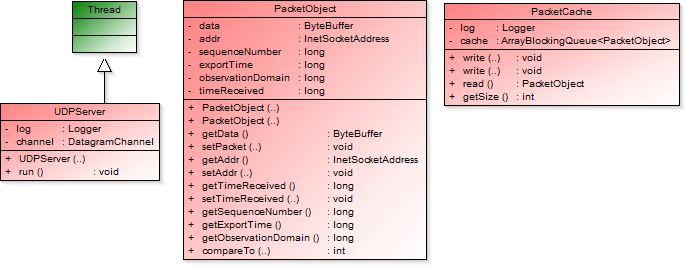
\includegraphics[width=1.0\textwidth]{collecting1_class}
\caption{Diagram tried prvej f�zy zhroma��ovacieho procesu}\label{o:collecting1_class}
\end{figure}


\subsubsection{Trieda UDPServer}
Sl��i ako UDP server. Prij�ma UDP datagramy cez \verb|DatagramChannel| a uklad� ich do 
\verb|PacketCache|. 

\bigskip
\textbf{Kon�truktor} 

\textit{public \textbf{UDPServer}(int port)}

Kon�truktor inicializuje \verb|DatagramChannel|, nastav� mu blokovac� re�im a privia�e ho k~portu 
definovanom v~konfigura�nom s�bore, ktor� mu je predan� ako parameter. Nastav� meno vl�kna.\\
\textbf{Parametre:} \\
\emph{int} port - ��slo portu

\bigskip
\textbf{Met�dy}

\textit{public void \textbf{run}()}

Hlavn� met�da vl�kna. Pokia� ned�jde k~preru�eniu, prij�ma cez vytvoren� kan�l d�ta od export�ra. 
Prijate d�ta obal� do objektu \verb|ByteBuffer| a pred� ich spolu s �asom prijatia a IP adresou a 
portom export�ra met�de \emph{write()}, ktor� ich zap��e do \verb|PacketCache|.


\textit{public void \textbf{cleanUp}()}

T�to met�da zru�� �istiace vl�kno pre UDP Template Cache. Je volan� pri preru�en� tohto vl�kna.

\begin{figure}[ht!]
\centering
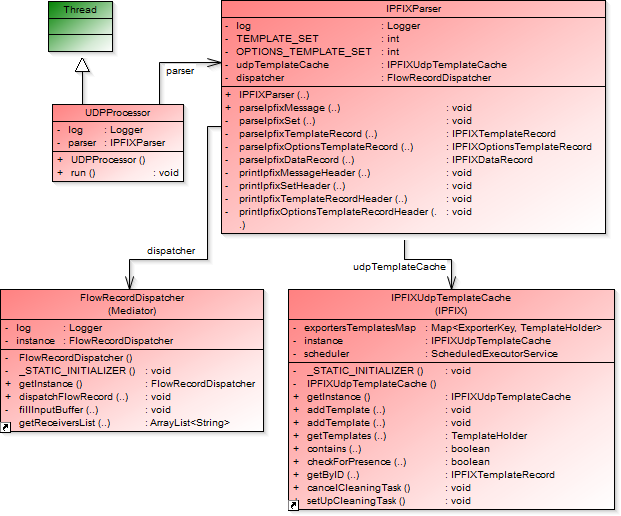
\includegraphics[width=1.0\textwidth]{collecting2_class}
\caption{Diagram tried druhej f�zy zhroma��ovacieho procesu}\label{o:collecting2_class}
\end{figure}
%---------

\subsubsection{Trieda IpfixParser}
T�to trieda sa pou��va na parsovanie IPFIX spr�v a ich spracovanie. V porovnan� s verziou 
v aplik�cii JXColl bola pre�isten�. Boli vypusten� sekcie spracov�vaj�ce TCP a SCTP spojenia. 
Z�sadnej�ia zmena pri�la na v�stupe z triedy. Sparsovan� d�tov� z�znamy s� zabalen� do vytvoren�ho 
objektu triedy 
\verb|IPFIXFlowRecord|, spolu s pr�slu�nou �abl�nou a hlavi�kou prijatej IPFIX spr�vy. Vytvoren� 
z�znam o toku je spolu s re�azcom predstavuj�cim zdroj z�znamu (v tomto pr�pade \uv{export�r})
posunut� triede \verb|FlowRecordDispatcher|.




% --------------------- EXPORTING ---------------------------

\subsection{Bal�k sk.tuke.cnl.bm.Mediator.exporting}

Diagram tried exportovacieho procesu je na Obr. \ref{o:exporting_class}.

\begin{figure}[ht!]
\centering
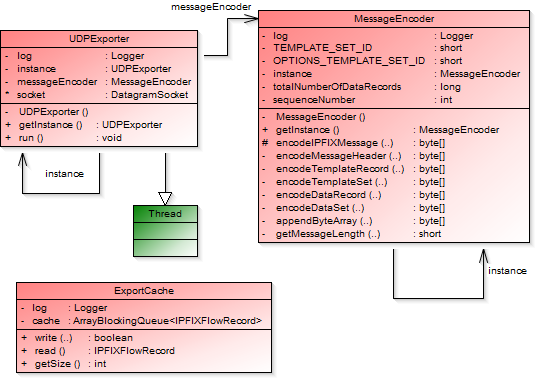
\includegraphics[width=1.0\textwidth]{exporting_class}
\caption{Diagram tried exportovacieho procesu}\label{o:exporting_class}
\end{figure}

\subsubsection{Trieda ExportCache}

Anal�gia k triede \verb|IPInputBuffer|. Reprezentuje exportovaciu cache, ktor� je synchronizovan� a 
jej implement�cia je FIFO front typu \verb|ArrayBlockingQueue|.

\textbf{Met�dy:}

\emph{public static boolean \textbf{write}(IPFIXFlowRecord flowRecord)}

Zapisuje z�znamy o tokoch do frontu. Ak je front pln�, z�znam sa zahadzuje.\\
\textbf{Parametre:}\\
\emph{IPFIXFlowRecord} flowRecord - z�znam o toku\\
\textbf{N�vratov� hodnota:}\\
Pravdivostn� hodnota pod�a toho, �i z�znam bol, alebo nebol zap�san� do cache.\\



\emph{public static IPFIXFlowRecord \textbf{read}()}

Pre��ta a zma�e vrchol frontu. Ak je front pr�zdny �ak� dokia� sa tam nejak� element neprid�.\\
\textbf{N�vratov� hodnota:}\\
Objekt triedy \verb|IPFIXFlowRecord|.\\
\textbf{H�d�e:}\\
\verb|InterruptedException| - Ak nastala chyba pri synchronizovan� vl�kien, alebo ak bolo vl�kno preru�en� 
po�as �akania.\\



\emph{public static int \textbf{getSize}()}

\textbf{N�vratov� hodnota:}\\
Vracia po�et elementov v cache.



\subsubsection{Trieda MessageEncoder}

Trieda sl��i na zak�dovanie resp. zabalenie z�znamu o toku do IPFIX paketu pod�a �pecifik�cie v RFC 5101 
a RFC 5102.\\
\\

\textbf{Met�dy:}


\emph{public static MessageEncoder \textbf{getInstance}()}

\textbf{N�vratov� hodnota:}\\
Met�da vracia jedine�n� in�tanciu objektu triedy pod�a n�vrhov�ho vzoru \emph{Singleton}.\\



\emph{protected byte[] \textbf{createIPFIXMessage}(IPFIXFlowRecord flowRecord)}

Na z�klade z�znamu o toku vytv�ra pr�d bytov z IPFIX spr�vy. Vola jednotlive met�dy, ktor� robia 
�iastkov� �lohy ako zak�dovanie s�d, hlavi�ky a podobne.\\
\textbf{Parametre:}\\
\emph{IPFIXFlowRecord} flowRecord - z�znam o toku\\
\textbf{N�vratov� hodnota:}\\
Pole bytov pr�du IPFIX spr�vy.\\



\emph{private byte[] \textbf{encodeMessageHeader}(IPFIXMessage.IPFIXMessageHeader header, short length)}

Zak�duje hlavi�ku IPFIX spr�vy.\\
\textbf{Parametre:}\\
\emph{IPFIXMessage.IPFIXMessageHeader} header - hlavi�ka, ktor� sa m� zak�dova�\\
\emph{short} length - celkov� d�ka IPFIX spr�vy\\
\textbf{N�vratov� hodnota:}\\
Pole bytov pr�du hlavi�ky IPFIX spr�vy.\\



\emph{private byte[] \textbf{encodeTemplateRecord}(IPFIXTemplateRecord templateRecord)}

Zak�duje z�znam �abl�ny.\\
\textbf{Parametre:}\\
\emph{IPFIXTemplateRecord} templateRecord - z�znam �abl�ny, ktor� sa m� zak�dova�\\
\textbf{N�vratov� hodnota:}\\
Pole bytov pr�du z�znamu �abl�ny.\\



\emph{private byte[] \textbf{encodeTemplateSet}(byte[] templateRecordBytes)}

Zak�duje sadu �abl�n.\\
\textbf{Parametre:}\\
\emph{byte[]} templateRecordBytes - pole bytov pr�du z�znamov �abl�ny, ktor� obsahuje sada �abl�ny\\
\textbf{N�vratov� hodnota:}\\
Pole bytov pr�du sady �abl�n.\\



\emph{private byte[] \textbf{encodeDataRecord}(IPFIXDataRecord dataRecord)}

Zak�duje d�tov� z�znam.\\
\textbf{Parametre:}\\
\emph{IPFIXDataRecord} dataRecord - d�tov� z�znam, ktor� sa m� zak�dova�\\
\textbf{N�vratov� hodnota:}\\
Pole bytov pr�du d�tov�ho z�znamu.\\


\emph{private byte[] \textbf{encodeDataSet}(ByteArrayOutputStream dataRecordsStream, int templateID)}

Zak�duje d�tov� sadu.\\
\textbf{Parametre:}\\
\emph{ByteArrayOutputStream} dataRecordsStream - pr�d bytov d�tov�ch z�znamov, ktor� obsahuje sada �abl�ny\\
\emph{int} templateID - ID prisl�chaj�cej �abl�ny \\
\textbf{N�vratov� hodnota:}\\
Pole bytov pr�du d�tovej sady.



\emph{private byte[] \textbf{appendByteArray}(byte[] first, byte[] second)}

Pomocn� met�da, ktor� na koniec prv�ho po�a bytov pripoj� druh� pole bytov .\\
\textbf{Parametre:}\\
\emph{byte[]} first - prve pole bytov \\
\emph{byte[]} second - druhe pole bytov\\
\textbf{N�vratov� hodnota:}\\
Pole bytov v�sledn�ho po�a.\\


\emph{private short \textbf{getMessageLength}(byte[] templateSetBytes, byte[] dataSetBytes, byte[] optionsTemplateSetStream)}

Vracia celkov� d�ku IPFIX spr�vy.\\
\textbf{Parametre:}\\
\emph{byte[]} templateSetBytes - pole bytov sady �abl�n\\
\emph{byte[]} dataSetBytes - pole bytov d�tovej sady\\
\emph{byte[]} optionsTemplateSetStream - pole bytov sady �abl�n mo�nost�\\
\textbf{N�vratov� hodnota:}\\
Celkov� d�ka IPFIX spr�vy, vr�tane hlavi�ky. N�vratov� typ je \emph{short}.



\subsubsection{Trieda UDPExporter}


Trieda je samostatn�m vl�knom, z�znamy o toku ��ta z ExportCache. Tie potom po�le triede 
\verb|MessageEncoder|, ktor� ich zabal� do IPFIX spr�v. Zak�dovan� spr�vy exportuje kolektoru na IP 
adresu a port, ktor� s� definovan� v konfigura�nom s�bore. \\

\textbf{Kon�truktor:}

\emph{private \textbf{UDPExporter}()}

Bezparametrick� kon�truktor. Vola rodi�ovsk� kon�truktor s parametrom svojho mena. Potom sa pok�si 
vytvori� socket pomocou triedy \verb|DatagramSocket|.\\

\textbf{Met�dy:}

\emph{public static MessageEncoder \textbf{getInstance}()}

\textbf{N�vratov� hodnota:}\\
Met�da vracia jedine�n� in�tanciu objektu triedy pod�a n�vrhov�ho vzoru \emph{Singleton}.\\


\emph{public void \textbf{run}()}

Hlavn� met�da vl�kna. Dokia� nie je vl�kno preru�en�, cyklicky ��ta z�znamy o toku z ExportCache.
Prostredn�ctvom triedy \verb|MessageEncoder| vytvor� zo z�znamu o toku v�stupn� pr�d bytov. 
Ten spolu s d�kou pr�du, IP adresou a portom zabal� do paketu - objektu triedy \verb|DatagramPacket|.
Vzniknut� paket odo�le.



% --------------------- EXCEPTIONS ---------------------------

\subsection{Bal�k sk.tuke.cnl.bm.exceptions}

Bal�k obsahuje triedy v�nimiek �pecifick�ch pre Medi�tor. V�etky v�nimky dedia od hlavnej triedy 
v�nimiek - \verb|MediatorException|.




\clearpage
\section{Preklad programu}

\subsection{Zoznam zdrojov�ch textov}
Zdrojov� texty s� k~dispoz�cii v~pr�lohe diplomovej pr�ce.

\noindent S� k~dispoz�cii tieto zdrojov� texty:

\begin{verbatim}
- bal�k sk.tuke.cnl.bm.Mediator:
   Config.java
   Default.java
   DropsCounter.java
   FlowRecordDispatcher.java
   IPLoader.java
   Mediator.java
   Support.java
- bal�k sk.tuke.cnl.bm.Mediator.IPFIX:
   ExporterKey.java
   FieldSpecifier.java
   IPFIXDataRecord.java
   IPFIXDecoder.java
   IPFIXElements.java
   IPFIXEncoder.java
   IPFIXFlowRecord.java
   IPFIXMessage.java
   IPFIXOptionsTemplateRecord.java
   IPFIXSet.java
   IPFIXTemplateRecord.java
   IpfixUdpTemplateCache.java
   TemplateHolder.java
- bal�k sk.tuke.cnl.bm.Mediator.IntermediateProcesses:
   AIntermediateProcess.java
   ExampleProcess.java
   IPInputBuffer.java
- bal�k sk.tuke.cnl.bm.Mediator.collecting:
   IPFIXParser.java
   PacketCache.java
   PacketObject.java
   UDPProcessor.java
   UDPServer.java
- bal�k sk.tuke.cnl.bm.Mediator.exporting:
   ExportCache.java
   MessageEncoder.java   
   UDPExporter.java
- bal�k sk.tuke.cnl.bm.exceptions:
   DataException.java
   DataFormatException.java
   EncodingException.java
   IPLoaderException.java
   MediatorException.java
   OutOfBoundsException.java
   TemplateException.java
\end{verbatim}



\subsection{Po�iadavky na technick� prostriedky pri preklade}

Preklad programu si vy�aduje nasledovn� hardv�rov� konfigur�ciu:
\begin{itemize}
  \item CPU Intel Pentium III 1Ghz alebo ekvivalent
  \item opera�n� pam� 512MB
  \item pevn� disk s~1GB vo�n�ho miesta
  \item sie�ov� karta 100Mb/s
\end{itemize}
\noindent




\subsection{Po�iadavky na programov� prostriedky pri preklade}
\begin{itemize}
\item opera�n� syst�m GNU/Linux s~verziou jadra 2.6 a vy��ou 
\item Java Runtime Environment (JRE) verzie 1.7.0\_03 a~vy��ej
\item kni�nice dod�van� na in�tala�nom m�diu
\end{itemize}




\subsection{N�v�znos� na in� programov� produkty}

Program umo��uje sprostredkovanie spr�v medzi merac�m/exportovac�m procesom a zhroma��ovac�m procesom 
IPFIX architekt�ry, ktor� bud� n�sledne vyhodnoten� pr�slu�n�mi aplik�ciami. Je implement�ciou 
\emph{(IP Flow Information Export (IPFIX) Mediation Problem)} v architekt�re SLAmeter.
Z~toho vypl�va jeho n�v�znos� na merac�/exportovac� proces - BEEM a zhroma��ovac� proces - JXColl 
(alebo in� implement�cie t�chto procesov).




\subsection{Vlastn� preklad}

Preklad programu spo��va v~nakop�rovan� zdrojov�ch s�borov a~spusten� kompil�tora jazyka
Java s~potrebn�mi parametrami a~parametrom classpath nastaven�m na pr�davn� kni�nice.
Odpor��a sa pou�i� v� ob��ben� java IDE, kde sta�� jednoducho nastavi� verziu JDK na 7.0
alebo vy��ie a~do cesty classpath prida� cesty ku v�etk�m potrebn�m kni�niciam. V~prostred�
NetBeans IDE potom sta�� klikn�� na tla�idlo \textit{Clean and Build}.




\subsection{Vytvorenie in�tala�n�ho DEB s�boru}
Sta�� spusti� skript \texttt{buildDeb.sh}, ktor� sa nach�dza v~prie�inku /deb.

\begin{center}
\texttt{sh buildDeb.sh }
\end{center}

V�stupom tohto skriptu je s�bor s~n�zvom \texttt{debian.deb}, ktor� m��me n�sledne premenova� pod�a verzie Medi�tora 
(napr�klad na mediator\_1.0\_i386.deb). 
Tento skript vykon�va nasledovn�:

\begin{enumerate}
\item v~pr�pade, ak neexistuje prie�inok debian, extrahuje ho z~arch�vu debian.tar.gz, inak tento krok presko��
\item skop�ruje bin�rny s�bor z~projektu do DEB bal��ka (predpoklad� sa, �e bol program kompilovan� v~Netbeans IDE pomocou Clean and Build tla�idla)
\item skop�ruje konfigura�n� s�bor z~projektu do DEB bal��ka
\item skop�ruje IPFIX defini�n� s�bor z~projektu do DEB bal��ka
\item vyma�e pr�padn� do�asn� s�bory z~DEB bal��ka
\item vygeneruje MD5 kontroln� s��ty pre v�etky s�bory DEB bal��ka
\item zabezpe�� maxim�lnu kompresiu manu�lov�ch str�nok a changelog s�borov
\item skop�ruje bin�rny s�bor z~projektu do DEB bal��ka a nastav� mu pr�va na vykon�vanie
\item vytvor� samotn� DEB bal��ek
\item over� ho pomocou programu lintian - ten vyp��e pr�padne varovania a/alebo chyby
\item archivuje vytvoren� DEB bal��ek do arch�vu debian.tar.gz
\end{enumerate}

Pred spusten�m skriptu je nutn� skompilova� Medi�tor pomocou Netbeans IDE tla�idlom \textit{Clean and Build}. 
Pr�padn� zmeny control alebo changelog s�boru, manu�lov�ch str�nok je nutn� vykona� ru�ne. 
Manu�lov� str�nky je vhodn� upravi� pomocou programu \textit{GmanEdit} . Po spusten� skriptu sa vytvor� 
DEB bal��ek s~n�zvom \texttt{debian.deb}. Ten je vhodn� premenova� pod�a aktu�lnej verzie. 
Vytvor� sa aj arch�v \texttt{debian.tar.gz}, ktor� obsahuje najaktu�lnej�iu adres�rov� �trukt�ru 
DEB bal��ka pre bud�ce vyu�itie (ak neexistuje prie�inok debian, vytvor� sa extrakciou z~tohto arch�vu). 
Ak je potrebn� len aktualizova� k�d, sta�� spusti� skript a ten sa o~v�etko postar�, pri�om vytvor� aj 
adres�r debian. S�bory mo�no v~�om upravova� a� k�m nie je v�etko pod�a predst�v. Ak je v�etko hotov�, 
v~Netbeans IDE je potrebn� vymaza� prie�inok debian (vykon� sa SVN DELETE, namiesto oby�ajn�ho 
odstr�nenia zo s�borov�ho syst�mu) a projekt ''commitn��''. \citep{jxcoll_sp, ado_dp}


\subsection{Opis zn�mych ch�b}
V~s��asnosti nie s� zn�me �iadne v�ne chyby.


\newpage
\section{Zhodnotenie rie�enia}
%Hlavn�m cie�om pr�ce bolo zv��i� interoperabilitu s~in�mi IPFIX rie�eniami pomocou zv��enia konformity so �tandardom IPFIX. 
%V~pr�ci boli vyrie�en� probl�my, ktor� doteraz znemo��ovali dek�dovanie viacer�ch z�znamov sade, informa�nc�ch elementov s~variabilnou d�kou, informa�n�ch elementov s~redukovan�m k�dovan�m alebo niektor�ch predt�m neimplementovan�ch d�tov�ch typov. 
%
%S��as�ou pr�ce bolo roz��renie podpory prenosu �dajov o~tokoch prostredn�ctvom transportn�ch protokolov TCP a SCTP, �o zvy�uje mo�nosti
%nasadenia n�stroja BasicMeter aj v~podmienkach s~vy��ou n�chylnos�ou na pre�a�enie v~siet�. 
%
%Mo�nosti bud�ceho v�voja zhroma��ovacieho procesu n�stroja BasicMeter predstavuje implement�cia podpory pre d�tov� typy umo��uj�ce
%prenos �trukt�rovan�ch d�t a podpora pre zabezpe�en� pripojenia od export�rov.
%


\clearpage
\addcontentsline{toc}{section}{\numberline{}Zoznam pou�itej literat�ry}
\begin{thebibliography}{999}

\harvarditem{Kobayashi, Claise}{2010}{rfc5982}
KOBAYASHI, A. -- CLAISE, B. et al.: \emph{IP Flow Information Export (IPFIX) Mediation: Problem Statement.} 
RFC 5982. 2010

\harvarditem{Kobayashi et al.}{2011}{rfc6183}
KOBAYASHI, A. et al.: \emph{IP Flow Information Export (IPFIX) Mediation: Framework.} 
RFC 6183. 2011

\harvarditem{Sadasivan, et al.}{2009}{rfc5470}
SADASIVAN, G. et al.: \emph{Architecture for IP Flow Information Export} 
RFC 5470. 2009

\harvarditem{Claise}{2004}{rfc3954}
CLAISE, B.: \emph{Cisco Systems NetFlow Services Export Version 9.} 
RFC 3954. 2004

\harvarditem{Vere���k}{2012}{jxcoll_sp}
VERE���K, T.: Optimaliz�cia zhroma��ovacieho procesu n�stroja BasicMeter, 2012,
Diplomov� pr�ca, Pr�loha A, Syst�mov� pr�ru�ka JXColl v3.9, KPI FEI TU, Ko�ice

\harvarditem{Pek�r}{2009}{ado_bc}
PEK�R, A.: Meranie prev�dzkov�ch parametrov siete v~re�lnom �ase, 2009,
Bakal�rska pr�ca, KPI FEI TU, Ko�ice

\harvarditem{Pek�r}{2011}{ado_dp}
PEK�R, A.: Optimaliz�cia zhroma��ovacieho procesu n�stroja BasicMeter, 2011,
Diplomov� pr�ca, KPI FEI TU, Ko�ice

\end{thebibliography}
%


\end{document}
%%